\section{Electronics}
\subsection{Powersupply}
One of the tasks of the project was to create a power supply for the FPGA board and the external components. This supply should take in a 15 V signal and divide it into 3 different voltage levels, namely a 5 V for the FPGA, a 6 V for powering the servo motor and a 12 V for powering the LEDs. The requirements for the project can be seen in table \ref{tab::power_req}. This should be soldered on a PCB made from scratch using Eagle, a CAD program for circuit design. The schematic of the board can be seen on figure \ref{fig::sch_power}, drawn in Eagle.
\subsubsection{Regulators}
\begin{wraptable}{r}{5cm}
\caption{Voltage and current requirements for the powersupply.}
\label{tab::power_req}
 \vspace{5 pt}
 \begin{tabular}{ccc}
  Voltage & Current & Tolerance \\
 \toprule
  12 V & 1 A & N/A \\
  6 V & 1.5 A & N/A \\
  5 V & 0.5 A & $\pm\ 1.5 \%$ \\
  \bottomrule
 \end{tabular}
\end{wraptable}
The 12 V and the 6 V supply is made with linear regulators, whereas the 5 V is a switching regulator. The 5V, driving the FPGA needs to be a lot more efficient than the others, due to it not being able to drive the FPGA properly if not efficient, and therefore a switching regulator was chosen. The linear regulators, L7806CV and the LM7812 are both rated to maximum giving out the required values, so the thing is just to dimension the capacitors on the output of the regulators. These are there in order to eliminate voltage spikes from the load. A standard\footnote{Ref to Practical Electronics page 702} for the output is $0.1 \mu F$.

\begin{figure}[H]
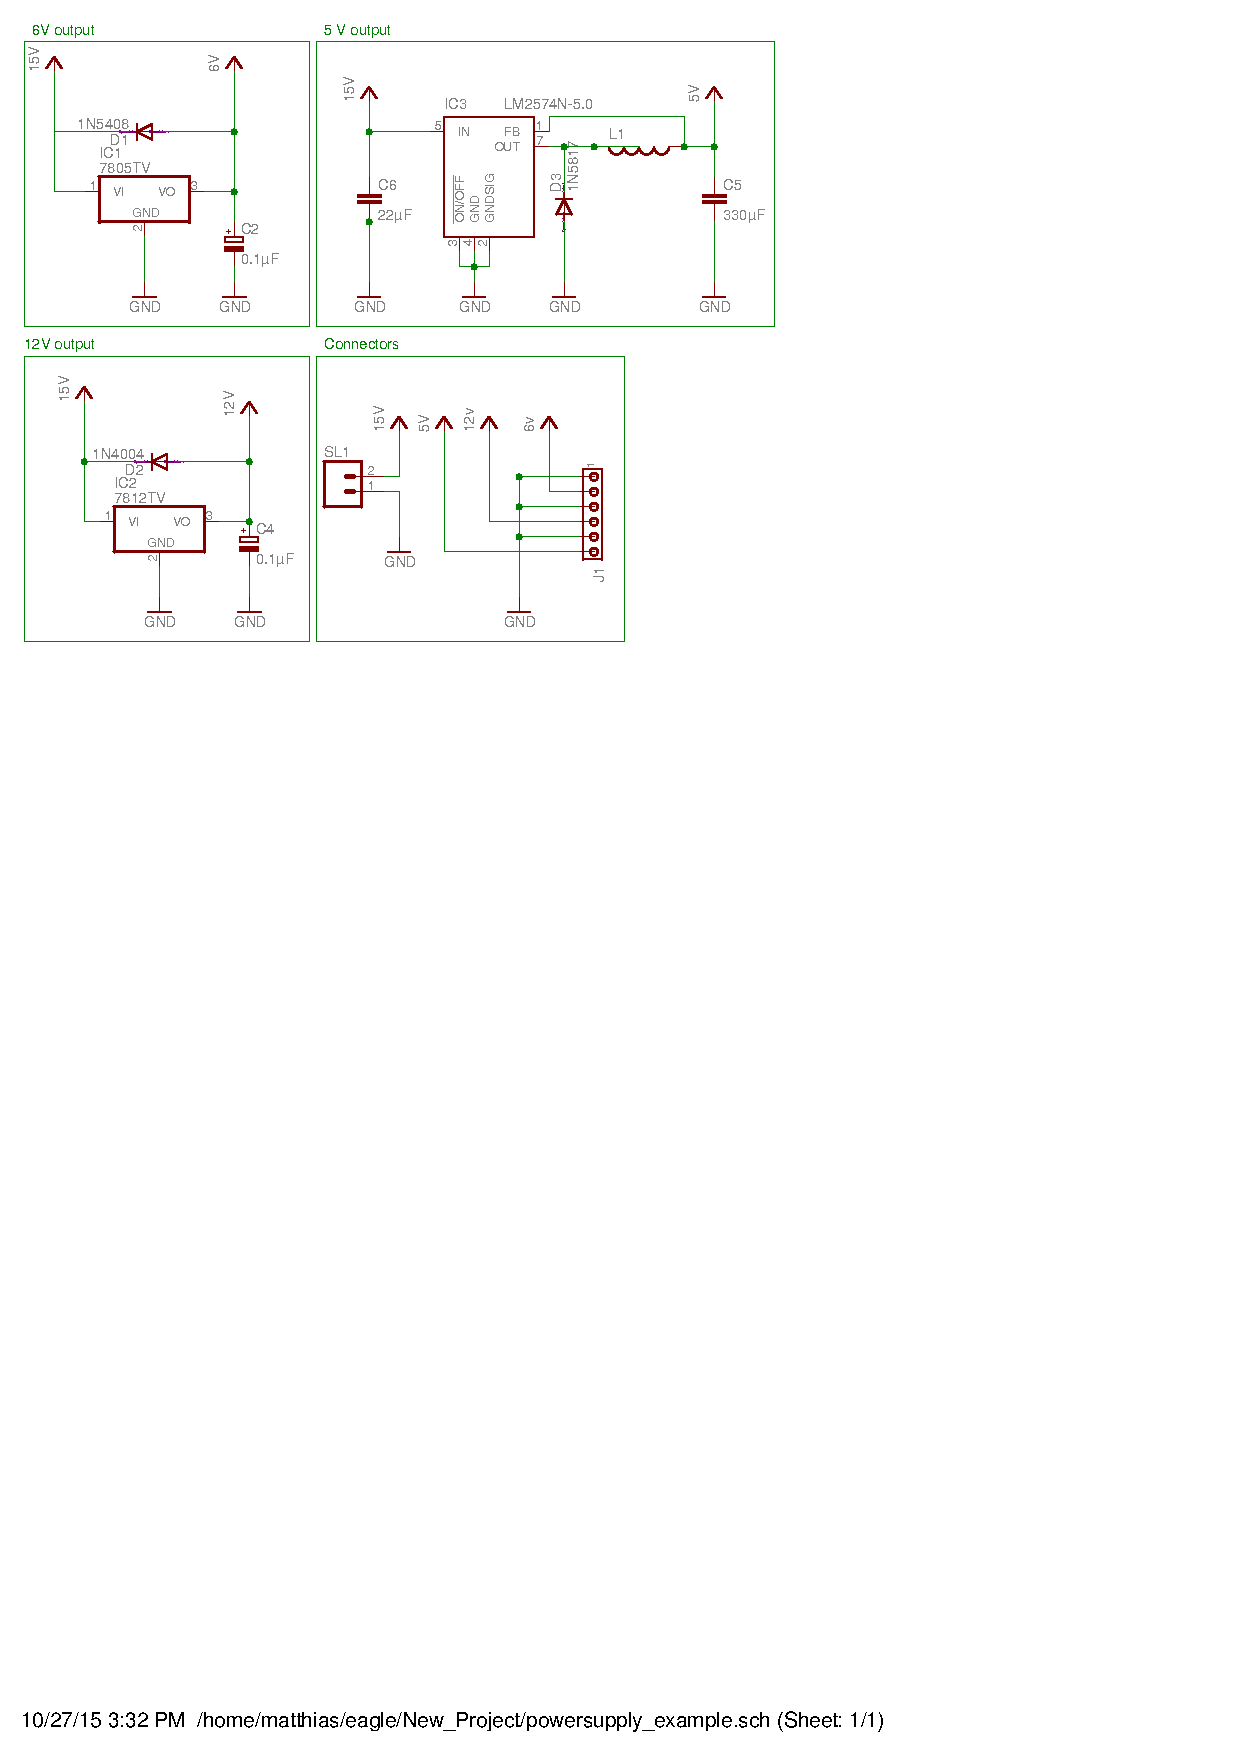
\includegraphics[scale=0.8,trim={0 19cm 0 0}]{img/powersupply.pdf}
\caption{Schematic diagram of power supply}
\label{fig::sch_power}
\end{figure}
\todo[inline]{Uddyb dette afsnit hvis nødvendigt med mere teori omkring regulatorer}
It is a bit different for the switching regulator. There is a inductor, whose value was chosen from figure 26 in the datasheet\footnote{datasheet for the LM2574}. Given the input voltage of 15 V and the max current drawn, 0.5 $\mu A$, the value of the inductor should be 330 $\mu H$. The output capacitor size is chosen so that the output voltage does not change significantly. In the datasheet for the LM2574 \footnote{datasheet for the LM2574} a value of 220 $\mu F$ is stated to be typical so this will also be used in this project. A diode is placed in between the regulator and inductor to protect the regulator against the inductor suddenly drawing a lot of current.

\subsubsection{Heat}
One of the problems when designing the circuit, is that the linear regulators, in order to convert 15V 1A to, say 6V 1.5A, some energy has to disappear from the system, in the form of heat. With the 6V case it is $(15V - 6V)\cdot 1.5A\ =\ 13.5\ W$. In the beginning it was assumed that adding heat sinks was not necessary, however after trying to draw max current from the 6V supply, i.e 1.5A, it shut down rather quickly. Therefore it was chosen to add a heat sink. 
\todo[inline]{Beskrive forhold ved belastning efter heat sinks er sat på.}
\todo[inline]{Lav nye test af powersupply}

\subsubsection{PCB design}
The components described above, put together as seen in the block diagram in figure \ref{fig::sch_power}, should be put on a PCB, in a reasonable way. One of the things that were taken into account when designing the PCB was, in order to save space, instead of having one capacitor on the each of the regulator input, the 15V input was put roughly in the middle of the regulators with only one input capacitor

\begin{figure}
\centering
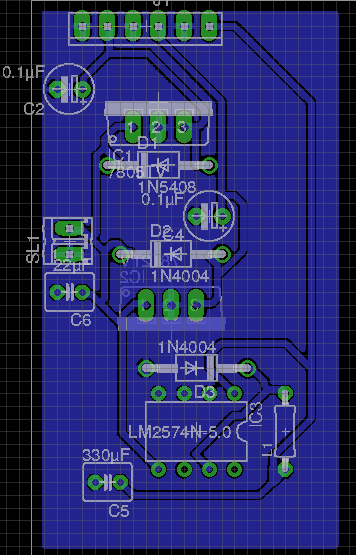
\includegraphics[scale=0.5]{img/pcb_power.png}
\caption{PCB design of the power supply made in Eagle} 
\label{fig::pcb_power}
\end{figure}